\documentclass[tikz,border=2pt]{standalone}
\usepackage{amsmath,amssymb}
\usepackage{tikz}
\usetikzlibrary{arrows.meta}

\begin{document}
% Six four-hour intervals with requirements d = (4,8,10,7,12,4); a bus starting in interval i
% works intervals i and i+1, so interval i is served by x_{i-1} + x_i buses (x_0 = x_6).
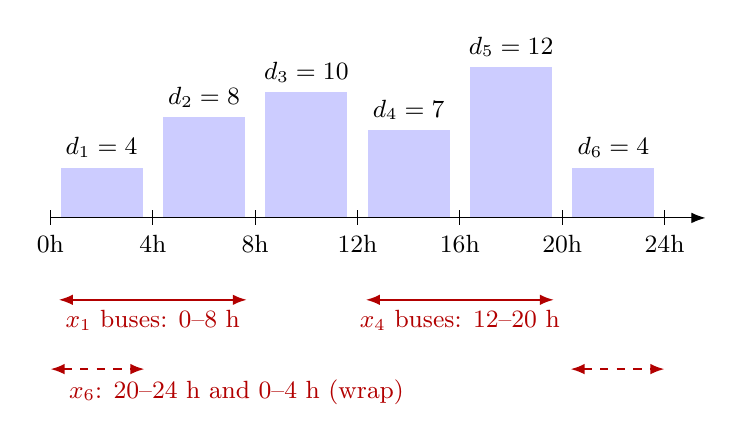
\begin{tikzpicture}[every node/.style={font=\small}, >={Latex[length=1.8mm]}, x=1.3cm, y=0.16cm]
	\foreach \i/\d in {1/4, 2/8, 3/10, 4/7, 5/12, 6/4} {
		\fill[blue!20] ({\i-0.9},0) rectangle ({\i-0.1},\d);
		\node[anchor=south] at ({\i-0.5},\d) {$d_\i=\d$};
	}
	\draw[->] (0,0) -- (6.4,0);
	\foreach \i/\l in {0/0, 1/4, 2/8, 3/12, 4/16, 5/20, 6/24} {\draw (\i,0.6) -- (\i,-0.6) node[below] {\l h};}
	\draw[<->, red!70!black, thick] (0.08,-6.5) -- (1.92,-6.5) node[midway, below] {$x_1$ buses: 0--8 h};
	\draw[<->, red!70!black, thick] (3.08,-6.5) -- (4.92,-6.5) node[midway, below] {$x_4$ buses: 12--20 h};
	\draw[<->, red!70!black, thick, dashed] (5.08,-12) -- (6.0,-12);
	\draw[<->, red!70!black, thick, dashed] (0,-12) -- (0.92,-12) node[midway, below, anchor=north west, xshift=-14pt] {$x_6$: 20--24 h and 0--4 h (wrap)};
	\end{tikzpicture}
\end{document}
